\newpage
{\bfseries МРНТИ 06.73.45}

\sectionwithauthors{К.Ж.Садвокасова, А.С.Бактымбет, Р.К.Садвокасов, А.К.Алпысбаева С.Рейдолда}{ДЕНЕЖНАЯ СИСТЕМА НЕЗАВИСИМОГО КАЗАХСТАНА: СТАНОВЛЕНИЕ И
НАПРАВЛЕНИЯ ДАЛЬНЕЙШЕГО РАЗВИТИЯ}

\begin{center}
{\bfseries \textsuperscript{1}К.Ж.Садвокасова, \textsuperscript{1}А.С.Бактымбет, \textsuperscript{2}Р.К.Садвокасов, \textsuperscript{1}А.К.Алпысбаева \textsuperscript{1}С.Рейдолда}

\textsuperscript{1}Казахский университет технологии и бизнеса, Астана,
Казахстан,

\textsuperscript{2}Евразийский национальный университет им.Л.Н.Гумилева,
Астана, Казахстан

Корреспондент-автор: ksadvokas@mail.ru
\end{center}

В 2023 году исполнилось~ровно~30 лет со дня принятия государственных
символов Республики Казахстан и 30 лет независимой денежной системе
Казахстана как суверенного государства. Уважение к Отчизне, трепетное
отношение к родной земле начинается с уважения к национальным
государственным символам, которые являются~~главными атрибутами
суверенитета страны, важнейшим инструментом укрепления национального
духа и общественного согласия, а также патриотического воспитания и
развития современной национальной экономики.~Таким же непременным
атрибутом суверенного государства является - независимая, устойчивая
денежная и финансовая система Республики Казахстан. Так как от состояния
денежной системы зависит успешное развитие национальной экономики.
Каждое суверенное государство имеет свою денежную систему. Под денежной
системой принято понимать форму организации денежного обращения в
стране, исторически сложившуюся и закрепленную национальным
законодательством. Составной частью денежной системы является
национальная валюта, которая в то же время относительно самостоятельна.
Денежные системы многих ныне развитых стран берут свое начало в
XVI--XVII веках, в период формирования национальных рынков и укрепления
государственной власти. Поэтому можно сказать, что современные денежные
системы различных стран имеют длительную историю, свои национальные
исторические и экономические особенности. В связи с этим фактором можно
сказать, что современный Казахстан сравнительно молодое государство. И
Казахстан не стал исключением по созданию своей независимой денежной
системы и не избежал ошибок, поскольку является довольно молодым
государством. Поэтому важно рассмотреть основные этапы становления и
развития независимой национальной денежной системы Казахстана.

{\bfseries Ключевые слова:} денежная система, элементы денежной системы,
национальная валюта, государство, финансовая система.

\begin{center}
{\large\bfseries ТӘУЕЛСІЗ ҚАЗАҚСТАННЫҢ АҚША ЖҮЙЕСІ: ҚАЛЫПТАСУЫ ЖӘНЕ ОДАН ӘРІ ДАМУ БАҒЫТТАРЫ}

{\bfseries \textsuperscript{1}Қ. Ж. Сәдуақасова,
\textsuperscript{1}А.С.Бақтымбет, \textsuperscript{2}Р.К.Сәдуақасов, \textsuperscript{1}А.К.Алпысбаева,
\textsuperscript{1}С.Рейдолда}

\textsuperscript{1}Қазақ технология және бизнес университеті, Астана,
Қазақстан,

\textsuperscript{2} Л.Н.Гумилев атындағы Еуразия ұлттық университеті,
Астана, Қазақстан,

e-mail: ksadvokas@mail.ru
\end{center}

2023 жылы Қазақстан Республикасының Мемлекеттік рәміздерінің
қабылданғанына тура 30 жыл және Қазақстанның егемен мемлекет ретіндегі
тәуелсіз ақша жүйесіне 30 жыл толды. Отанға деген құрмет, туған жерге
деген құрмет елдің егемендігінің басты атрибуттары, ұлттық рух пен
қоғамдық келісімді нығайтудың, сондай-ақ қазіргі ұлттық экономиканы
патриоттық тәрбиелеу мен дамытудың маңызды құралы болып табылатын ұлттық
мемлекеттік рәміздерді құрметтеуден басталады. Қазақстан Республикасының
тәуелсіз, тұрақты ақша және қаржы жүйесі - егеменді мемлекеттің дәл
осындай ажырамас атрибуты болып табылады. Өйткені ұлттық экономиканың
табысты дамуы ақша жүйесінің жағдайына байланысты. Әрбір егеменді
мемлекеттің өзіндік ақша жүйесі бар. Ақша жүйесі деп тарихи қалыптасқан
және ұлттық заңнамамен бекітілген елдегі ақша айналымын ұйымдастыру
формасы түсініледі. Ақша жүйесінің ажырамас бөлігі-бұл салыстырмалы
түрде тәуелсіз ұлттық валюта. Көптеген дамыған елдердің ақша жүйелері
XVI--XVII ғасырларда, ұлттық нарықтардың қалыптасуы мен мемлекеттік
биліктің нығаюы кезеңінде пайда болды. Сондықтан әр түрлі елдердің
қазіргі ақша жүйелерінің ұзақ тарихы, ұлттық тарихи және экономикалық
ерекшеліктері бар деп айтуға болады. Осы факторға байланысты қазіргі
Қазақстан салыстырмалы түрде жас мемлекет деп айтуға болады. Қазақстан
өзінің тәуелсіз ақша жүйесін құруда да ерекшелік болған жоқ және
қателіктерден қашқан жоқ, өйткені ол өте жас мемлекет. Сондықтан
Қазақстанның тәуелсіз ұлттық ақша жүйесінің қалыптасуы мен дамуының
негізгі кезеңдерін қарастыру маңызды.

{\bfseries Түйін сөздер}: ақша жүйесі, ақша жүйесінің элементтері, ұлттық
валюта, мемлекет, қаржы жүйесі.

{\large\bfseries THE MONETARY SYSTEM OF INDEPENDENT KAZAKHSTAN: FORMATION AND DIRECTIONS OF FURTHER DEVELOPMENT}

\begin{center}
{\bfseries \textsuperscript{1}K.J.Sadvokasova, \textsuperscript{1}A.S.
Baktymbet , \textsuperscript{2}R.K.Sadvokasov, \textsuperscript{1}A.K.Alpysbaeva, \textsuperscript{1}S.
Reidolda}

\textsuperscript{1} Kazakh University of Technology and Business,
Astana, Kazakhstan,

\textsuperscript{2} L.N.Gumilev Eurasian National University, Astana,
Kazakhstan,

e-mail: ksadvokas@mail.ru
\end{center}

In 2023, exactly 30 years have passed since the adoption of the state
symbols of the Republic of Kazakhstan and 30 years of the independent
monetary system of Kazakhstan as a sovereign state. Respect for the
Motherland, reverent attitude to the native land begins with respect for
national state symbols, which are the main attributes of the
country\textquotesingle s sovereignty, an important tool for
strengthening the national spirit and social harmony, as well as
patriotic education and the development of a modern national economy.
The same indispensable attribute of a sovereign state is an independent,
stable monetary and financial system of the Republic of Kazakhstan.
Since the successful development of the national economy depends on the
state of the monetary system. Each sovereign state has its own monetary
system. The monetary system is usually understood as a form of
organization of monetary circulation in the country, historically
established and enshrined in national legislation. An integral part of
the monetary system is the national currency, which at the same time is
relatively independent. The monetary systems of many now developed
countries originate in the XVI--XVII centuries, during the formation of
national markets and the strengthening of state power. Therefore, it can
be said that modern monetary systems of various countries have a long
history, their own national historical and economic characteristics. In
connection with this factor, we can say that modern Kazakhstan is a
relatively young state. And Kazakhstan was no exception in creating its
own independent monetary system and did not avoid mistakes, since it is
a fairly young state. Therefore, it is important to consider the main
stages of the formation and development of an independent national
monetary system in Kazakhstan.

{\bfseries Keywords}: monetary system, elements of the monetary system,
national currency, state, financial system.

\begin{multicols}{2}
{\bfseries Введение.} В этой связи необходимо рассмотреть становление
денежной системы Республики Казахстан, так как наше государство является
сравнительно молодым. А сам процесс становления денежной системы не
избежал ряд ошибок, трудностей и даже парадоксов. Как известно
элементами денежной системы являются следующее:

- национальная денежная единица;

- виды денежных знаков;

- масштаб цен;

- эмиссионный механизм.

Денежная система Республики Казахстан была построена на основе денежной
планово-командной экономики СССР. Поэтому денежная система Республики
Казахстан унаследовала все трудности и проблемы денежной системы
советского государства. Основной денежной единицей был советский рубль,
который имел золотое содержание 0, 987412 г. золота. В обращении
находились казначейские билеты Основой достоинством в 1, 3, 5 рублей и
банковские билеты достоинством в 10, 25, 50, 100 рублей и разменная
монета. Причем уже позже после развала СССР не советские рубли, а
российские рубли имели хождение на территории Республики Казахстан
вплоть до 15 ноября 1993 года -даты введения национальной валюты
«тенге», хотя как известно независимость наша страна обрела еще в 1991
году. Поэтому важно рассмотреть и проанализировать основные этапы
развития и совершенствования денежной системы Казахстана. Так как
политический суверенитет не означает еще экономический суверенитет.

{\bfseries Материалы и методы.} При написании статьи были использованы
следующие методы: методы сравнительного анализа, метод диалектического
материализма, эмпирические методы, сравнительно-исторический метод.

Цель исследования заключается в анализе основных этапов развития
национальной денежной системы Казахстана, как суверенного государства и
влияние на ее развитие не только экономических факторов, но и
политических. Всегда ли Национальный банк Казахстана принимал
своевременные и решительные меры по борьбе с инфляцией?

Гипотеза строится на том, что несмотря на заявления руководства
Казахстана, что проводим независимую экономическую политику, тем не
менее влияние внешних факторов сильно влияет на уровень инфляции в
стране и соответственно на состояние экономики.

Новизна данной статьи заключается в том, что до сих пор не были
исследованы причины инфляции на разных этапах развития рыночной
экономики и причины несвоевременного реагирования на эти процессы
главного банка страны -- Национального банка Республики Казахстан, как
проводника соотвествующей денежно-кредитной политики.

Как уже было сказано денежная система различных стран имеет свои
национальные и исторические особенности. Такие особенности имеет и
Республика Казахстана. К ним можно отнести следующие факты:

Во - первых, независимость Республики Казахстан была объявлена
16.12.1991 года. Однако мы не можем утверждать, что уже в 1991 году
Казахстан имел независимую самостоятельную денежную систему, так как на
этот период отсутствовали отдельные элементы денежной системы, а именно
- национальная единица денежного счета. Так как в обращении находилась
по сути дела валюта другого государства - российский рубль, эмитируемый
Центральным банком Российской Федерации.

Во - вторых, поскольку обращался российский рубль вплоть до 15 ноября
1993 года, то виды денежных знаков, выпускаемых, в обращении естественно
устанавливались не Национальным банком Республики Казахстан, а
Центральным банком Российской Федерации.

Поэтому можно сказать Республика Казахстан объявив последней из всех
республик СССР политическую независимость не был подлинно экономически
независимым государством

В - третьих, поскольку Национальный банк Республики Казахстан не
выпускал денег в обращении, то он не выполнял свою главную функцию-
эмиссионную. И это притом, что согласно Закону еще Казахской ССР с 1990
года, в нашем государстве функционировала двухуровневая банковская
система.

В - четвертых, отсутствовала полноценная законодательно - нормативная
база, так как Законы РК «О Нацбанке РК», и «О банках и банковской
деятельности» от 1993 года были не совершенны, поскольку были приняты
еще до введения национальной валюты. Также эти законы не полностью
отражали роль, функции и полномочия банков в рыночных отношениях.

В - пятых, надо отметить, что введение национальной валюты в Республике
Казахстан происходило в экстренном порядке. Так как, в августе 1993 года
правительство России в одностороннем порядке нарушило договор о едином
экономическом пространстве с единой валютой, введя в обращении денежные
знаки нового дизайна, которые имели хождение только на территории
Российской Федерации. Тем самым произошло фактическое разделение
денежных систем России и Казахстана. И день 15 ноября в Республики
Казахстан является днем национальной валюты и профессиональным
праздником работников финансовой, бюджетной, налоговой,
кредитно-банковской систем.

В - шестых, Закон РК «О денежной системе Республики Казахстан» был
принят только в декабре 1993 года. Этот закон устанавливает правовые
основы и формы организации денежного обращения, включающий в себя
официальную денежную единицу, порядок чеканки монет и эмиссии денежных
знаков. В данном законе говорится, что единственным законным платежным
средством на территории Республики Казахстан является -- тенге. Однако
нужно отметить, что на практике часто это положение нарушается, особенно
СМИ, где публикуются объявления о купле--продаже и цена товара, услуг
или недвижимости указывается в иностранной валюте.

В - седьмых, более совершенные Законы Республики Казахстан «О Нацбанке»
и «О банках и банковской деятельности» были приняты в 1995 году, где
Национальному банку Республики Казахстан придан соответствующий статус
главного Центрального банка и четко разграничены функции и операции БВУ.

В - восьмых, сам 1993 год в истории Казахстана ознаменовался как год
введения национальной валюты, то за тем следующий 1994 год -год
обвального падения национальной валюты тенге по отношению к доллару. На
момент введения национальной валюты 1 доллар США равнялся 4 тенге 65
тиын, а к концу 1994 года - почти 60 тенге. В 1994 году страна пережила
галопирующую, а затем гиперинфляцию и стагфляцию, сопровождавшуюся
спадом производства и ростом безработицы.

В - девятых, 1995 год -- год начала проведения Национальным банком
Республики Казахстан жесткой денежно-кредитной политики -«кредитной
рестрикции». Первые результаты были получены в 1996 году. 1996 год
переломный год в дальнейшем развитии денежной системы Республики
Казахстан, так как положено начало макроэкономической стабилизации.
Национальный банк Республики Казахстан становится подлинным центральным
банком нашего государства.

В - десятых, в 1999 году был введен свободный плавающий обменный
валютный курс, что явилось правильным решением, после известного
«черного августа» 1998 года в России. В Республике Казахстан создана
собственная банковская фабрика и монетный двор, которые полностью
обеспечивают потребности экономики в наличных деньгах. В последние годы
Национальный банк Республики Казахстан выпускает в обращение банкноты
нового дизайна. Ветхие деньги достоинством с 1 тенге до 50 тенге изъяты
из обращения и заменены металлическими монетами.

Большое значение Национальный банк Республики Казахстан придает монетной
продукции. Если в 1993 году были выпущены бумажные монеты, то сегодня
выпускаются монеты из различных сплавов, включая коллекционные и
инвестиционные, золотые и серебряные монеты, которые продаются по
рыночной цене\emph{.} Здесь уместно вспомнить, что первые подобные
монеты для Казахстана были изготовлены Австрийским монетным двором.
Первые бумажные деньги - тенге печатались в Англии и доставлялись
спецсамолетами в Казахстан {[}1{]}.

Опыт развитых стран, в частности США, говорит о том, что к созданию
независимой денежной системы каждая страна пришла через «свои» трудности
и проблемы. Любопытен тот факт, что еще в XVIII веке денежное обращение
на американском континенте обслуживалось иностранными деньгами -
английскими фунтами стерлингов и испанскими серебряными долларами. В
1785 году конгресс США объявил национальной денежной единицей - доллар.
Но денежное обращение в США было децентрализовано, банкноты выпускались
частными банками. К примеру, в 1859 году в обращении находились 5 400
видов банкнот, выпущенных более чем 1000 банками. И только в 1913 году
федеральным актом, была учреждена федеральная резервная система (ФРС),
которая включает 12 федеральных резервных банков. А доллар по сей день
является свободно конвертируемой валютой и выступает в роли мировых
денег. А многие страны ведут борьбу за дедолларизацию экономики, в том
числе и Казахстан.

\begin{figure}[H]
	\centering
	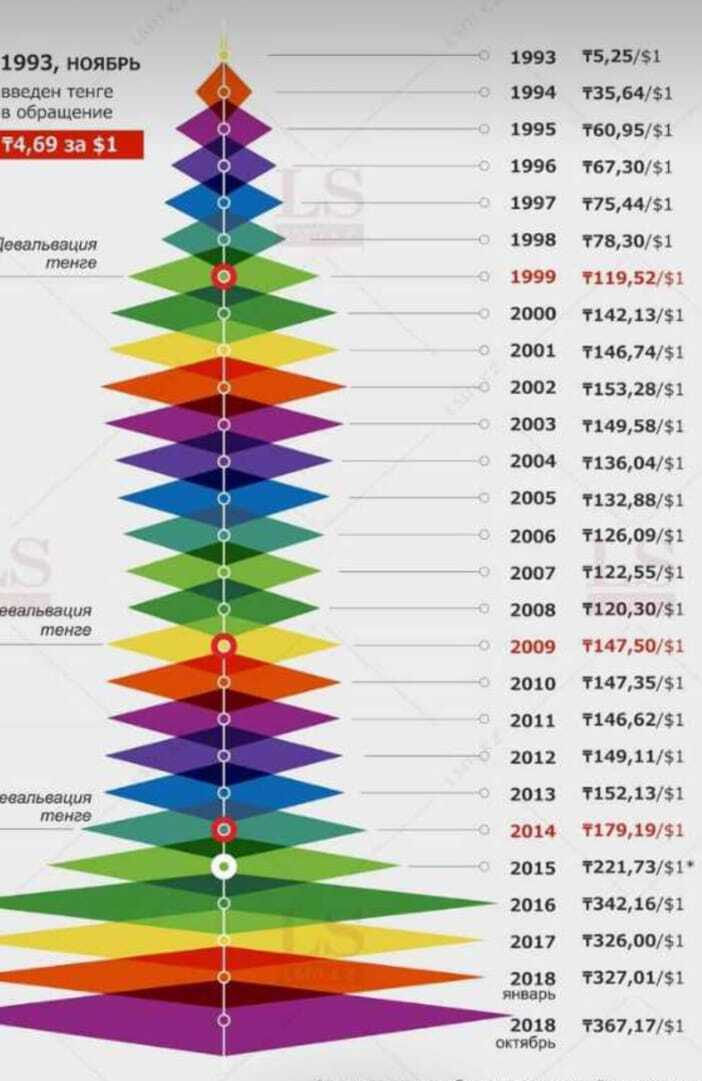
\includegraphics[width=0.4\textwidth]{assets/1117}
	\caption*{Рис.1 - Динамика девальвации тенге за период с 1993 по 2018 годы}
\end{figure}

Поэтому можно сказать, что за короткий период становления независимого
государства, Казахстан создал национальную денежную систему, а
банковская система Республики Казахстан была признана одной из лучших
среди стран СНГ. А Национальный банк Республики Казахстан подчинил свою
деятельность главной задаче - обеспечению устойчивости национальной
валюты и стабильности цен.

Однако надо сказать, что по истечении 30 лет независимости Казахстана
главный банк страны плохо справляется со своими главными функциями. За
что подвергся заслуженной критики со стороны Президента Республики
Казахстана Токаева К.К. в Послании от 1 сентября 2022 г. {[}2{]}.

Динамика девальвации тенге по отношению к доллару в период с 1993 года
по 2018 год приведена на рисунке 1{[}3{]}. Таким образом, если на момент
введения национальной валюты-тенге \$1 стоил 4,69 тенге. То на
1.11.2022г. \$1= 475 тенге. Инфляция составила 101,3 \%.

{\bfseries Результаты обсуждения.} По итогам 2020 года, впервые за 10 лет
индустриализации, вклад обрабатывающей промышленности в развитие
экономики превысил долю горнодобывающей отрасли. Среднесрочная цель - к
2025 году увеличить экспорт обрабатывающей промышленности в 1,5 раза, до
24 млрд долларов, а производительность труда - на 30\% {[}2 {]}.

Вместе с тем, Президент Токаев К.К. подверг резкой критики деятельность
Национального банка Казахстан, который плохо справляется со своей
главной функцией денежно-кредитного регулирования экономики. Несмотря на
то, что Национальный Банк Казахстана самостоятельно, а также
взаимодействуя с другими государственными органами, разрабатывает и
осуществляет меры, направленные на обеспечение стабильности финансовой
системы:

1) проводит регулярный мониторинг макроэкономических и макрофинансовых
факторов, влияющих на стабильность финансовой системы;

2) формирует макропруденциальную политику;

3) предоставляет займы последней инстанции в порядке, предусмотренном
законодательством;

4) проводит мониторинг системных рисков финансовой системы;

5) в случае возникновения или угрозы возникновения системного
финансового кризиса

самостоятельно или совместно с Правительством Республики Казахстан
вводит ограничения на проведение отдельных видов банковских и других
операций финансовыми организациями.

Также им были отмечены, что Казахстан столкнулся с неконтролируемым
ростом инфляции. Национальный банк, Правительство Республики Казахстан
оказались бессильными перед ней, сославшись на мировые тенденции.
Подобного рода отговорки высвечивают уязвимость национальной экономики.
Возникает еще один вопрос: в чем тогда состоит роль наших
профессиональных экономистов? Главная задача Национального банка и
Правительства - это возвращение инфляции в коридор 4-6\% {[}2{]}.

Что касается инфляции, то по данным Бюро национальной статистики
Агентства по стратегическому планированию и реформам Республики
Казахстан, в августе 2021 года инфляция составила 0,5\% (в августе 2020
года -- 0,1\%). Годовая инфляция сложилась на уровне 8,7\% (в декабре
2020 года -- 7,5\%). В структуре инфляции цены на продовольственные
товары в годовом выражении повысились на 11,4\%, непродовольственные
товары -- на 7,3\%, платные услуги -- на 6,6\%. В августе 2021 года
количественная оценка ожидаемой через год инфляции по результатам опроса
населения составила 8,8{]}. Теперь о немонетарных составляющих инфляции.
Главная из них - цены на продукты питания.
\end{multicols}

\begin{figure}[H]
	\centering
	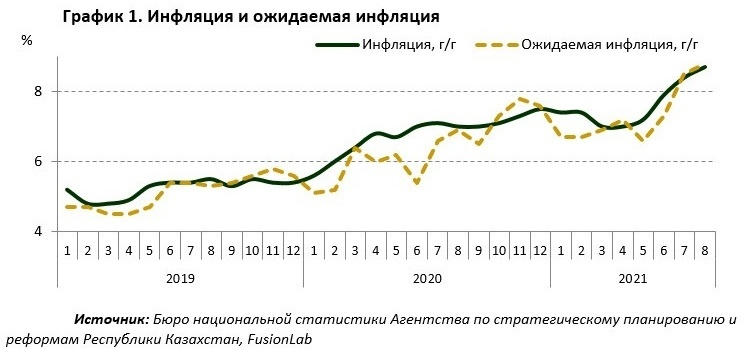
\includegraphics[width=0.8\textwidth]{assets/1118}
	\caption*{Рис. 2 -- Фактическая и ожидаемая инфляция в РК, в \% \_\_\_\_\_\_\_\_\_фактическая инфляция \_ \_ \_ \_ ожидаемая инфляция}
\end{figure}

\begin{multicols}{2}
Целью денежно-кредитной политики Национального Банка является удержание
инфляции в пределах установленных ориентиров. Среднесрочный таргет по
инфляции установлен на уровне 3-4\%. В целях обеспечения
сбалансированного экономического развития Национальный Банк стремится
осуществить постепенное снижение инфляции до данного уровня. Для этого
целевые ориентиры установлены следующим образом:

А) на 2021-2022 годы -- 4-6\%;

Б) на 2023-2024 годы -- 4-5\%;

В) с 2025 года -- 3-4\% {[}1 {]}.
\end{multicols}

\begin{figure}[H]
	\centering
	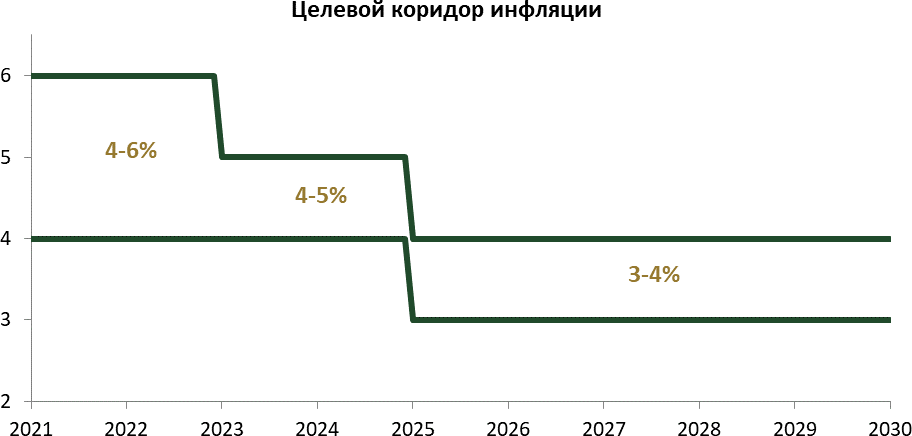
\includegraphics[width=0.6\textwidth]{assets/1119}
	\caption*{Рис. 3 -- Целевые ориентиры по инфляции до 2025 года}
	\caption*{(Источник: данные сайта Нацбанка РК-www.nationalbank.kz)}
\end{figure}

\begin{multicols}{2}
Однако эти целевые ориентиры по инфляции не были выдержаны по разным
причинам, в том числе из-за непредвиденных событий как начало СВО России
на Украине. За короткое время наша страна стала транзитной для беженцев
из России. Так россияне по данным Национального банка Казахстана завезли
в нашу страну около 50 млрд.рублей, которые подхлестнули цены на рынке
продовольствия, рынке недвижимости и рынке потребительских услуг и
соответственно инфляцию в стране, которая подскочила до 18\% в 2022 году
вместо планируемых 4-46\%.

В то же время на рынке труда продолжает расти число закрываемых
предприятий и число временно приостановленных, что говорит о
определенном кризисе в производственной сфере.

В~настоящее время в~Казахстане действуют почти 346,6 тыс. компаний.
В~их~число входят 172,2 тыс. активных юридических лиц (+1\% за~год),
53,8 тыс. вновь зарегистрированных (+11,9\%) и~120,6 тыс. временно
приостановленных (+16,5\%). Это следует из~данных бюро национальной
статистики.

Если рассматривать последнюю категорию предприятий, больше всего
временно приостановленных субъектов работали в~торговле, ремонте авто
и~мотоциклов (35,6 тыс.), в~строительстве (23 тыс.)
и~в~профессиональной, научной и~технической деятельности (7~729).

Также на~паузу поставили работу юридических лиц в~обрабатывающей
промышленности - в~сельском, лесном, рыбном хозяйстве, в~области
административного и~вспомогательного обслуживания, а~также транспорте
и~складировании. Помимо этого, в~Казахстане на~1~октября 2021 года
в~процессе ликвидации находится 5~421 предприятие {[}3{]}.

Это говорит о серьезном снижении роли банков в экономике. Достаточно для
этого сравнить показатели банков трех стран ЕАЭС -- Казахстана, России и
Беларуси. В результате реализации антикризисных мер общим объемом 6,3
трлн тенге в экономике возникла избыточная денежная масса. Но существуют
ниши, в которые эти средства не поступают. Банки второго уровня не
вкладываются в небольшие проекты, особенно на селе {[}4{]}.

В Казахстане и Российской Федерации процесс оптимизации
институциональной структуры продолжается. В частности, за период с 1
января 2013 года по 1 января 2020 года количество зарегистрированных и
имеющих право на осуществление банковских операций банков России
снизилось в два раза (с 923 до 402). За анализируемый период банковская
система Казахстана сократилась на 11 банков или почти на треть их общего
числа к уровню 2013 года, сохранив 27 банков второго уровня.

В целом, данный тренд соответствует глобальным тенденциям в сфере
финансового посредничества, которая находится под воздействием феномена
«цифровой компрессии». Индикаторами происходящих процессов являются не
только консолидация рынка, но и общее сокращение его объемов и
доходности бизнеса. Например, только в 2018 году в Европе прекратили
работу 330 банков или 5\% всего сегмента {[}5,6{]}.

Что же касается роли банковской системы в экономике, измеряемая как
отношение совокупных активов к ВВП, является индикатором эффективности
выполнения банками функции финансового посредника. В экономиках развитых
стран данный индикатор достигает размера ВВП. Надо отметить, что
банковский сектор России в данном случае является примером соответствия
лучшим мировым практикам, однако последние четыре года показатель
соотношения активов к ВВП также снижается (Таблица 2). Роль банковского
сектора Беларуси в финансировании экономики не только не достигает
порогового значения 60\% объёма ВВП, но имеет тенденцию к ежегодному
снижению.
\end{multicols}

\begin{table}[H]
\caption*{Таблица 1 -- Совокупные активы банковского сектора в \% к ВВП}
\centering
\begin{tabular}{|llllllll|}
\hline
\multicolumn{1}{|l|}{Страна} & \multicolumn{1}{l|}{2014} & \multicolumn{1}{l|}{2015} & \multicolumn{1}{l|}{2016} & \multicolumn{1}{l|}{2017} & \multicolumn{1}{l|}{2018} & \multicolumn{1}{l|}{2019} & 2020 \\ \hline
\multicolumn{1}{|l|}{Казахстан} & \multicolumn{1}{l|}{45,1} & \multicolumn{1}{l|}{46,3} & \multicolumn{1}{l|}{61,4} & \multicolumn{1}{l|}{57,6} & \multicolumn{1}{l|}{45,4} & \multicolumn{1}{l|}{40,8} & 39,6 \\ \hline
\multicolumn{1}{|l|}{Беларусь} & \multicolumn{1}{l|}{54,9} & \multicolumn{1}{l|}{55,2} & \multicolumn{1}{l|}{64,5} & \multicolumn{1}{l|}{67,2} & \multicolumn{1}{l|}{58,4} & \multicolumn{1}{l|}{53,9} & 54,6 \\ \hline
\multicolumn{1}{|l|}{Россия} & \multicolumn{1}{l|}{80,9} & \multicolumn{1}{l|}{99,6} & \multicolumn{1}{l|}{102,7} & \multicolumn{1}{l|}{93,01} & \multicolumn{1}{l|}{92,5} & \multicolumn{1}{l|}{90,2} & 88,3 \\ \hline
\multicolumn{8}{|l|}{Источник – {[}4,5,6{]}} \\ \hline
\end{tabular}
\end{table}

\begin{table}[H]
\caption*{Таблица 2 -- Казахстан в мировом рейтинге разведанных земных богатств}
\centering
\begin{tabular}{|llll|}
\hline
\multicolumn{2}{|l|}{Наименование} & \multicolumn{1}{l|}{Доля в \%} & Место в мире \\ \hline
\multicolumn{1}{|l|}{1} & \multicolumn{1}{l|}{Свинец} & \multicolumn{1}{l|}{22\%} & 1 \\ \hline
\multicolumn{1}{|l|}{2} & \multicolumn{1}{l|}{Цинк} & \multicolumn{1}{l|}{15,2} & 1 \\ \hline
\multicolumn{1}{|l|}{3} & \multicolumn{1}{l|}{Уран} & \multicolumn{1}{l|}{18,9} & 2 \\ \hline
\multicolumn{1}{|l|}{4} & \multicolumn{1}{l|}{Хромовые руды} & \multicolumn{1}{l|}{37,6} & 1 \\ \hline
\multicolumn{1}{|l|}{5} & \multicolumn{1}{l|}{Барит} & \multicolumn{1}{l|}{47,2} & 1 \\ \hline
\multicolumn{1}{|l|}{6} & \multicolumn{1}{l|}{Уголь} & \multicolumn{1}{l|}{3,1} & 6 \\ \hline
\multicolumn{1}{|l|}{7} & \multicolumn{1}{l|}{Нефть} & \multicolumn{1}{l|}{3,2} & 6 \\ \hline
\multicolumn{1}{|l|}{8} & \multicolumn{1}{l|}{\textbf{Золото}} & \multicolumn{1}{l|}{\textbf{2,70\%}} & \textbf{8} \\ \hline
\multicolumn{1}{|l|}{9} & \multicolumn{1}{l|}{\textbf{Серебро}} & \multicolumn{1}{l|}{\textbf{16\%}} & \textbf{2} \\ \hline
\multicolumn{1}{|l|}{10} & \multicolumn{1}{l|}{Медь} & \multicolumn{1}{l|}{7,1} & 3 \\ \hline
\multicolumn{1}{|l|}{11} & \multicolumn{1}{l|}{Никель} & \multicolumn{1}{l|}{1,4} & 12 \\ \hline
\multicolumn{1}{|l|}{12} & \multicolumn{1}{l|}{Кобальт} & \multicolumn{1}{l|}{3,9} & 5 \\ \hline
\multicolumn{1}{|l|}{13} & \multicolumn{1}{l|}{Бокситы} & \multicolumn{1}{l|}{1,4} & 10 \\ \hline
\multicolumn{1}{|l|}{14} & \multicolumn{1}{l|}{Железо} & \multicolumn{1}{l|}{6} & 5 \\ \hline
\multicolumn{1}{|l|}{15} & \multicolumn{1}{l|}{Марганец} & \multicolumn{1}{l|}{30} & 2 \\ \hline
\multicolumn{1}{|l|}{16} & \multicolumn{1}{l|}{Фосфориты} & \multicolumn{1}{l|}{4,5} & 6 и т.д. \\ \hline
\multicolumn{1}{|l|}{} & \multicolumn{1}{l|}{\begin{tabular}[c]{@{}l@{}}По размеру территории\\   Казахстан занимает\end{tabular}} & \multicolumn{1}{l|}{} & 9 место из 148 стран \\ \hline
\multicolumn{1}{|l|}{} & \multicolumn{1}{l|}{Население казахстана} & \multicolumn{1}{l|}{0,25} & От всего населения земли \\ \hline
\multicolumn{4}{|p{0.6\textwidth}|}{\textit{Примечание: по данным сайта Бюро национальной статистики Агентства по стратегическому планированию и реформам Республики Казахстан {[}Электронный ресурс{]}. - Режим доступа:http//www.zakon/kz}} \\ \hline
\end{tabular}
\end{table}

\begin{multicols}{2}
Для Казахстана данное значение составляет менее 40\% и находится на
критическом уровне, что свидетельствует о недостаточности ресурсов и
наличии внутренних системных структурных рисков банковской системы, не
позволяющих банкам наращивать объёмы привлекаемых ресурсов для
вовлечения их в экономический оборот.

Таким образом, можно сделать выводы, что в странах ЕАЭС есть
определенные трудности и несоответствие по ряду показателей, которые
нужно будет преодолеть в кратчайшие сроки, так как банковские системы
являются основным звеном финансового рынка{[}7,8,9{]}

Из данных таблицы 2 видно, что мы очень богатая страна природными и
сырьевыми ресурсами и можем построить успешную рыночную экономику с
устойчивой денежной системой и национальной валютой {[}10,11{]}.

{\bfseries Выводы.} Завершение перехода на режим полноценного инфляционного
таргетирования позволит создать благоприятные условия для устойчивого
роста диверсифицированной экономики, включающие высокий уровень доверия
к проводимой денежно-кредитной политике и, как следствие, национальной
валюте, стабилизацию инфляционных ожиданий, а также сохранение
плавающего курсообразования, которое будет способствовать устойчивости
платежного баланса и поддержанию достаточного уровня международных
резервов.

Денежно-кредитная политика, как один из элементов макроэкономической
политики государства, будет служить, в первую очередь, целям поддержания
и повышения благосостояния населения. Она продолжит обеспечивать
устойчивое функционирование экономики, и достижение общеэкономических
целей страны. Наиболее важным приоритетом денежно-кредитной политики
будет оставаться обеспечение стабильности цен и сглаживание циклических
колебаний экономической активности через воздействие процентных ставок
на спрос. Стабильность цен будет достигаться не только через снижение
фактической инфляции, но также посредством стабилизации ее долгосрочной
динамики. Стабильная и низкая инфляция позволит сохранить стоимость
активов населения и компаний, а также снизить связанные с ней
общественные издержки. Второй значимой целью Национального Банка будет
обеспечение финансовой стабильности. При возникновении рисков для
финансовой системы денежно-кредитная политика будет направлена на
повышение ее устойчивости {[}12{]}.
\end{multicols}

\begin{center}
{\bfseries Литература:}
\end{center}

\begin{noparindent}
1.Годовые отчёты Национального Банка РК за 2020-2022 годы //

https://nationalbank.kz/docid=31\&switch=russian.- Дата обращения
15.10.2023 г.

2.Послание Президента РК Токаева К.К. «Единство народа и системные
реформы - прочная основа процветания страны» от 1.09.2021 года
{[}Электронный ресурс{]}. - Режим доступа:http//www.zakon/kz- Дата
обращения 15.10.2023 г.

3.Бюро национальной статистики Агентства по стратегическому планированию
и реформам Республики Казахстан {[}Электронный ресурс{]}. - Режим
доступа:http//www.zakon/kz- Дата обращения 15.10.2023 г.

4.Банковский сектор Республики Беларусь {[}Электронный ресурс{]}. -
Режим доступа:http//www.nbrb.by- Дата обращения 15.10.2023 г.

5.Текущее состояние банковского сектора Республики Казахстан
{[}Электронный ресурс{]}. - Режим доступа:http//www.nationalbank.kz -
Дата обращения 15.10.2023 г.

6.Обзор банковского сектора Российской Федерации. {[}Электронный
ресурс{]}.- Режим доступа:http//www.cbr.ru- Дата обращения 01.11.2023 г.

7.Концепция развития финансового сектора Республики Казахстан до 2030
года: утв. постановлением Правительства Республики Казахстан 29 августа
2014, №954 // https://nationalbank.kz/?docid=382\&switch=russian.
25.12.2015.- Дата обращения 01.10.2023 г.

8.Sadvokassova К.Zh., Kodasheva G.S., Slyamova B.I. To the question of
transformation of banking activities in Kazakhstan into banking business
// Известия Национальной Академии наук Республики Казахстан. - 2018. -
№1(317). - C. 64-70.

9.Садвокасова К.Ж., Кодашева Г.С. Факторы, влияющие на развитие
банковской деятельности в Казахстане в условиях роста неопределённости
// Известия высших учебных заведений. Поволжский регион. Общественные
науки. -- 2017. -- №1(41). -- С. 167-176.

10.Парусимова Н.И., Садвокасова К.Ж., Кодашева Г.С. Банки Казахстана в
условиях экономической нестабильности // Интеллект. Инновации.
Инвестиции. -- 2016. -- №11. -- С. 60-66.

11.Садвокасова К.Ж. Влияние роста неопределенности на развитие
банковской деятельности в Казахстане: теория и практика:
Монография.-«ТОО Полиграфический центр «Индиго Принт», Астана,
2022.-156с.

12.Сратегия денежно-кредитной политики до 2030 г./Постановление Нацбанка
РК: http//www.nationalbank.kz- Дата обращения 03.12.2023
\end{noparindent}

\begin{center}
{\bfseries References}
\end{center}

\begin{noparindent}
1.Godovye otchjoty Nacional\textquotesingle nogo Banka RK za 2020-2022
gody //

https://nationalbank.kz/docid=31\&switch=russian.- Data
obrashhenija 15.10.2023 g.

2.Poslanie Prezidenta RK Tokaeva K.K. «Edinstvo naroda i sistemnye
reformy - prochnaja osnova procvetanija strany» ot 1.09.2021 goda
{[}Jelektronnyj resurs{]}. - Rezhim dostupa:http//www.zakon/kz- Data

obrashhenija 15.10.2023 g.

3.Bjuro nacional\textquotesingle noj statistiki Agentstva po
strategicheskomu planirovaniju i reformam Respubliki Kazahstan
{[}Jelektronnyj resurs{]}. - Rezhim dostupa:http//www.zakon/kz- Data
obrashhenija 15.10.2023 g.

4.Bankovskij sektor Respubliki Belarus\textquotesingle{} {[}Jelektronnyj
resurs{]}. - Rezhim dostupa:http//www.nbrb.by- Data

obrashhenija
15.10.2023 g.

5.Tekushhee sostojanie bankovskogo sektora Respubliki Kazahstan
{[}Jelektronnyj resurs{]}. - Rezhim dostupa: http//www.nationalbank.kz -
Data obrashhenija 15.10.2023 g.

6.Obzor bankovskogo sektora Rossijskoj Federacii. {[}Jelektronnyj
resurs{]}.- Rezhim dostupa:http//www.cbr.ru- Data obrashhenija
01.11.2023 g.

7.Koncepcija razvitija finansovogo sektora Respubliki Kazahstan do 2030
goda: utv. postanovleniem Pravitel\textquotesingle stva Respubliki
Kazahstan 29 avgusta 2014, №954 //
https://nationalbank.kz/?docid=382\&switch=russian. 25.12.2015.- Data
obrashhenija 01.10.2023 g.

8. Sadvokassova К.Zh., Kodasheva G.S., Slyamova B.I. To the question of
transformation of banking activities in Kazakhstan into banking business
// Izvestiya National Academy of Sciences of the Republic of Kazakhstan.
- 2018. - №1(317). - C. 64-70

9. Sadvokasova K.Zh., Kodasheva G.S. Faktory, vlijajushhie na razvitie
bankovskoj dejatel\textquotesingle nosti v Kazahstane v uslovijah rosta
neopredeljonnosti // Izvestija vysshih uchebnyh zavedenij. Povolzhskij
region. Obshhestvennye nauki. -2017. - №1(41). - S. 167-176.

10. Parusimova N.I., Sadvokasova K.Zh., Kodasheva G.S. Banki Kazahstana
v uslovijah jekonomicheskoj

nestabil\textquotesingle nosti // Intellekt.
Innovacii. Investicii. -2016. - №11.- S. 60-66.

11.Sadvokasova K.Zh. Vlijanie rosta neopredelennosti na razvitie
bankovskoj dejatel\textquotesingle nosti v Kazahstane: teorija i
praktika: Monografija.-«TOO Poligraficheskij centr «Indigo Print»,
Astana, 2022.-156s.

12.Srategija denezhno-kreditnoj politiki do 2030 g./Postanovlenie
Nacbanka RK: http//www.nationalbank.kz- Data obrashhenija 03.12.2023
\end{noparindent}

\emph{{\bfseries Сведения об авторах}}

\begin{noparindent}
Садвокасова К.Ж.- доктор экономических наук, профессор Казахского
университета технологии и бизнеса им. К.Кулажанова, Астана, Казахстан,
e-mail: ksadvokas@mail.ru;

Бактымбет А.С. -кандидат экономических наук, ассоциированный
профессор,Казахского университета

технологии и бизнеса им. К.Кулажанова, Астана, Казахстан,
e-mail:asem\_abs@mail.ru;

Садвокасов Р.К.- магистр экономических наук, главный специалист
Евразийского национального университета им. Л.Н. Гумилева, Астана,
Казахстан, e-mail:rustems@ mail.ru;

Алпысбаева А.К.- кандидат экономических наук, ассоциированный профессор
Казахского университета технологии и бизнеса им.К. Кулажанова, e-mail:
alpysbayeva.ainur77@mai.ru;

Рейдолда С. -магистр экономических наук, старший преподаватель
Казахского университета технологии и бизнеса им. К.Кулажанова, e-mail:
sau\_1981@mail.ru
\end{noparindent}

{\bfseries Information about the author}

\begin{noparindent}
Sadvokasova K.Zh. - Doctor of Economics, Professor of Kazakh University
of Technology and Business named after K.Kulazhanov, Astana, Kazakhstan,
e-mail: ksadvokas@mail.ru;

Baktymbet A.S. - Candidate of Economic Sciences, Associate Professor, of
the Kazakh University of Technology and Business named after
K.Kulazhanov, Astana, Kazakhstan, e-mail:asem\_abs@mail.ru;

Sadvokasov R.K. - Master of Economic Sciences, Chief Specialist of L.N.
Gumilev Eurasian National University, Astana, Kazakhstan,
e-mail:rustems@ mail.ru;

Alpysbaeva A.K.- Candidate of Economic Sciences, Associate Professor of
Kazakh University of Technology and Business named after K.Kulazhanov,
Astana, Kazakhstan, e-mail: ,alpysbayeva.ainur77@mail.ru;

Reidolda S. - magistr ekonomicheskikh nauk, senior teacher of Kazakh
University of Technology and Business named after K.Kulazhanov, Astana,
Kazakhstan, e-mail: sau\_1981@mail.ru
\end{noparindent}
